% Note that the a4paper option is mainly intended so that authors in
% countries using A4 can easily print to A4 and see how their papers will
% look in print - the typesetting of the document will not typically be
% affected with changes in paper size (but the bottom and side margins will).
% Use the testflow package mentioned above to verify correct handling of
% both paper sizes by the user's LaTeX system.
%
% Also note that the "draftcls" or "draftclsnofoot", not "draft", option
% should be used if it is desired that the figures are to be displayed in
% draft mode.
% conference
\documentclass[draftclsnofoot]{IEEEtran}
\usepackage{graphicx}
% Add the compsoc option for Computer Society conferences.

% Sin esto los captions no aparecen centrados, no se porque!!!
\usepackage{caption}

% If IEEEtran.cls has not been installed into the LaTeX system files,
% manually specify the path to it like:
% \documentclass[conference]{../sty/IEEEtran}


% *** CITATION PACKAGES ***
%
%\usepackage{cite}
% cite.sty was written by Donald Arseneau
% V1.6 and later of IEEEtran pre-defines the format of the cite.sty package
% \cite{} output to follow that of IEEE. Loading the cite package will
% result in citation numbers being automatically sorted and properly
% "compressed/ranged". e.g., [1], [9], [2], [7], [5], [6] without using
% cite.sty will become [1], [2], [5]--[7], [9] using cite.sty. cite.sty's
% \cite will automatically add leading space, if needed. Use cite.sty's
% noadjust option (cite.sty V3.8 and later) if you want to turn this off.
% cite.sty is already installed on most LaTeX systems. Be sure and use
% version 4.0 (2003-05-27) and later if using hyperref.sty. cite.sty does
% not currently provide for hyperlinked citations.
% The latest version can be obtained at:
% http://www.ctan.org/tex-archive/macros/latex/contrib/cite/
% The documentation is contained in the cite.sty file itself.


% *** GRAPHICS RELATED PACKAGES ***
%
\ifCLASSINFOpdf
  % \usepackage[pdftex]{graphicx}
  % declare the path(s) where your graphic files are
  % \graphicspath{{../pdf/}{../jpeg/}}
  % and their extensions so you won't have to specify these with
  % every instance of \includegraphics
  % \DeclareGraphicsExtensions{.pdf,.jpeg,.png}
\else
  % or other class option (dvipsone, dvipdf, if not using dvips). graphicx
  % will default to the driver specified in the system graphics.cfg if no
  % driver is specified.
  % \usepackage[dvips]{graphicx}
  % declare the path(s) where your graphic files are
  % \graphicspath{{../eps/}}
  % and their extensions so you won't have to specify these with
  % every instance of \includegraphics
  % \DeclareGraphicsExtensions{.eps}
\fi


% *** MATH PACKAGES ***
%
%\usepackage[cmex10]{amsmath}
% A popular package from the American Mathematical Society that provides
% many useful and powerful commands for dealing with mathematics. If using
% it, be sure to load this package with the cmex10 option to ensure that
% only type 1 fonts will utilized at all point sizes. Without this option,
% it is possible that some math symbols, particularly those within
% footnotes, will be rendered in bitmap form which will result in a
% document that can not be IEEE Xplore compliant!
%
% Also, note that the amsmath package sets \interdisplaylinepenalty to 10000
% thus preventing page breaks from occurring within multiline equations. Use:
%\interdisplaylinepenalty=2500
% after loading amsmath to restore such page breaks as IEEEtran.cls normally
% does. amsmath.sty is already installed on most LaTeX systems. The latest
% version and documentation can be obtained at:
% http://www.ctan.org/tex-archive/macros/latex/required/amslatex/math/


% *** SPECIALIZED LIST PACKAGES ***
%
%\usepackage{algorithmic}
% algorithmic.sty was written by Peter Williams and Rogerio Brito.
% This package provides an algorithmic environment fo describing algorithms.
% You can use the algorithmic environment in-text or within a figure
% environment to provide for a floating algorithm. Do NOT use the algorithm
% floating environment provided by algorithm.sty (by the same authors) or
% algorithm2e.sty (by Christophe Fiorio) as IEEE does not use dedicated
% algorithm float types and packages that provide these will not provide
% correct IEEE style captions. The latest version and documentation of
% algorithmic.sty can be obtained at:
% http://www.ctan.org/tex-archive/macros/latex/contrib/algorithms/
% There is also a support site at:
% http://algorithms.berlios.de/index.html
% Also of interest may be the (relatively newer and more customizable)
% algorithmicx.sty package by Szasz Janos:
% http://www.ctan.org/tex-archive/macros/latex/contrib/algorithmicx/


% *** ALIGNMENT PACKAGES ***
%
%\usepackage{array}
% Frank Mittelbach's and David Carlisle's array.sty patches and improves
% the standard LaTeX2e array and tabular environments to provide better
% appearance and additional user controls. As the default LaTeX2e table
% generation code is lacking to the point of almost being broken with
% respect to the quality of the end results, all users are strongly
% advised to use an enhanced (at the very least that provided by array.sty)
% set of table tools. array.sty is already installed on most systems. The
% latest version and documentation can be obtained at:
% http://www.ctan.org/tex-archive/macros/latex/required/tools/


%\usepackage{mdwmath}
%\usepackage{mdwtab}
% Also highly recommended is Mark Wooding's extremely powerful MDW tools,
% especially mdwmath.sty and mdwtab.sty which are used to format equations
% and tables, respectively. The MDWtools set is already installed on most
% LaTeX systems. The lastest version and documentation is available at:
% http://www.ctan.org/tex-archive/macros/latex/contrib/mdwtools/


% IEEEtran contains the IEEEeqnarray family of commands that can be used to
% generate multiline equations as well as matrices, tables, etc., of high
% quality.


%\usepackage{eqparbox}
% Also of notable interest is Scott Pakin's eqparbox package for creating
% (automatically sized) equal width boxes - aka "natural width parboxes".
% Available at:
% http://www.ctan.org/tex-archive/macros/latex/contrib/eqparbox/



% *** SUBFIGURE PACKAGES ***
%\usepackage[tight,footnotesize]{subfigure}
% subfigure.sty was written by Steven Douglas Cochran. This package makes it
% easy to put subfigures in your figures. e.g., "Figure 1a and 1b". For IEEE
% work, it is a good idea to load it with the tight package option to reduce
% the amount of white space around the subfigures. subfigure.sty is already
% installed on most LaTeX systems. The latest version and documentation can
% be obtained at:
% http://www.ctan.org/tex-archive/obsolete/macros/latex/contrib/subfigure/
% subfigure.sty has been superceeded by subfig.sty.


%\usepackage[caption=false]{caption}
%\usepackage[font=footnotesize]{subfig}
% subfig.sty, also written by Steven Douglas Cochran, is the modern
% replacement for subfigure.sty. However, subfig.sty requires and
% automatically loads Axel Sommerfeldt's caption.sty which will override
% IEEEtran.cls handling of captions and this will result in nonIEEE style
% figure/table captions. To prevent this problem, be sure and preload
% caption.sty with its "caption=false" package option. This is will preserve
% IEEEtran.cls handing of captions. Version 1.3 (2005/06/28) and later 
% (recommended due to many improvements over 1.2) of subfig.sty supports
% the caption=false option directly:
%\usepackage[caption=false,font=footnotesize]{subfig}
%
% The latest version and documentation can be obtained at:
% http://www.ctan.org/tex-archive/macros/latex/contrib/subfig/
% The latest version and documentation of caption.sty can be obtained at:
% http://www.ctan.org/tex-archive/macros/latex/contrib/caption/




% *** FLOAT PACKAGES ***
%
%\usepackage{fixltx2e}
% fixltx2e, the successor to the earlier fix2col.sty, was written by
% Frank Mittelbach and David Carlisle. This package corrects a few problems
% in the LaTeX2e kernel, the most notable of which is that in current
% LaTeX2e releases, the ordering of single and double column floats is not
% guaranteed to be preserved. Thus, an unpatched LaTeX2e can allow a
% single column figure to be placed prior to an earlier double column
% figure. The latest version and documentation can be found at:
% http://www.ctan.org/tex-archive/macros/latex/base/



%\usepackage{stfloats}
% stfloats.sty was written by Sigitas Tolusis. This package gives LaTeX2e
% the ability to do double column floats at the bottom of the page as well
% as the top. (e.g., "\begin{figure*}[!b]" is not normally possible in
% LaTeX2e). It also provides a command:
%\fnbelowfloat
% to enable the placement of footnotes below bottom floats (the standard
% LaTeX2e kernel puts them above bottom floats). This is an invasive package
% which rewrites many portions of the LaTeX2e float routines. It may not work
% with other packages that modify the LaTeX2e float routines. The latest
% version and documentation can be obtained at:
% http://www.ctan.org/tex-archive/macros/latex/contrib/sttools/
% Documentation is contained in the stfloats.sty comments as well as in the
% presfull.pdf file. Do not use the stfloats baselinefloat ability as IEEE
% does not allow \baselineskip to stretch. Authors submitting work to the
% IEEE should note that IEEE rarely uses double column equations and
% that authors should try to avoid such use. Do not be tempted to use the
% cuted.sty or midfloat.sty packages (also by Sigitas Tolusis) as IEEE does
% not format its papers in such ways.





% *** PDF, URL AND HYPERLINK PACKAGES ***
%
%\usepackage{url}
% url.sty was written by Donald Arseneau. It provides better support for
% handling and breaking URLs. url.sty is already installed on most LaTeX
% systems. The latest version can be obtained at:
% http://www.ctan.org/tex-archive/macros/latex/contrib/misc/
% Read the url.sty source comments for usage information. Basically,
% \url{my_url_here}.



% *** Do not adjust lengths that control margins, column widths, etc. ***
% *** Do not use packages that alter fonts (such as pslatex).         ***
% There should be no need to do such things with IEEEtran.cls V1.6 and later.
% (Unless specifically asked to do so by the journal or conference you plan
% to submit to, of course. )

% correct bad hyphenation here
\hyphenation{op-tical net-works semi-conduc-tor}

\begin{document}

\title{Future Virtual Particle Method for Pedestrian Navigation}

\author{
    \IEEEauthorblockN{Castiglione Gonzalo,}
    \IEEEauthorblockA{Instituto Tecnológico de Buenos Aires\\
    }
    \and
    \IEEEauthorblockN{Marseillan Agustin,}
    \IEEEauthorblockA{Instituto Tecnológico de Buenos Aires\\
    }
    \and
    \IEEEauthorblockN{Parisi Daniel,}
    \IEEEauthorblockA{Instituto Tecnológico de Buenos Aires\\
    }
}

% make the title area
\maketitle

\begin{abstract}
%\boldmath
Pedestrians are modeled as passive objects affected by repulsive and attractive forces in the Social Force Model (SFM). This force governed model leads to unnatural behaviors that don't resemble reality.
This paper presents an avoidance collision method based in pedestrian self governed decisions, by calculating the position of every pedestrian in the future, a given pedestrian can adjust his velocity vector to avoid collisions instead of a repulsive force.
\end{abstract}
% IEEEtran.cls defaults to using nonbold math in the Abstract.
% This preserves the distinction between vectors and scalars. However,
% if the journal you are submitting to favors bold math in the abstract,
% then you can use LaTeX's standard command \boldmath at the very start
% of the abstract to achieve this. Many IEEE journals frown on math
% in the abstract anyway.

% Note that keywords are not normally used for peerreview papers.
\begin{IEEEkeywords}
pedestrian, collision avoidance, future virtual particle, force model
\end{IEEEkeywords}




% For peer review papers, you can put extra information on the cover
% page as needed:
% \ifCLASSOPTIONpeerreview
% \begin{center} \bfseries EDICS Category: 3-BBND \end{center}
% \fi
%
% For peerreview papers, this IEEEtran command inserts a page break and
% creates the second title. It will be ignored for other modes.
\IEEEpeerreviewmaketitle

\section{Introduction}
\subsection{Motivation and previous work}

Navigation of biological, sinthetic or virtual agents is a relevant
problem in several fields such as pedestrian dynamics, moving robots
and animation of characters for videogames and motion pictures.

Modelling and simulating the displacement of agents through arbitrarily
complex environments may be stated in an hierarchical structure of
mechanisms depending mainly on the distance from the agent. This level
has been named, from closer to further, as operational (walking, lowest
level physical-computational model for displacement), tactical (way-finding,
route choice) and strategic (general activity planning) \cite{key-hoog2004}. 
These levels are not independent, factors affecting
one level may impact in the following and vice-versa, for example,
the route choice may vary due to congestion of agents produced from
previous route choice and walking behavior. Also, obstacles can impact
on the operational level or tactical level depending on the particular
geometry of the environment. The particular mechanism we want to address
is the avoidance of obstacles being fixed or moving (another agent)
which involves operational and tactical aspects of the navigation.

A general approach is to take an existing operational model and equip
it with a higher level model which allows better and smoother collision
avoidance behavior. Existing low level models can be taken from pedestrian
dynamics field and in general this models can be classified into rule
based and force based, discrete and continuous space description,
etc. \cite{key-scha2009}.

A famous example of continuous and force based model is the Social
Force Model \cite{key-helb1995, key-helb2000}. In this model the dynamic for
virtual pedestrians is derived from the Newton equation's considering
the total force exerted over each agent is the result of three forces:
Contact, Social and Driving Force. While the driving force points
towards the final objective of each pedestrian, the social force is
repulsive and acts as a kind of collision avoidance force. However
this social force term introduces several artifices in some configurations.
See for example Lakoba \cite{key-tara2005}, Parisi \cite{key-pari2009}.

Cellular automaton models make use of a spatial grid, which can be
occupied or empty, along with a set of rules determining the evolution
and conflict resolution of virtual pedestrians moving over the cells
of the grid. An emblematic cellular automaton model is the one proposed
by Kirchner and Schadschneider \cite{key-kirc2002}.

Hybrid models have also been proposed such as the Contractile Particle
Model \cite{key-pari2011} in which a continuous description
of the space is combined with a set of simple rules governing the
dynamics of the system.

The basic operational model -as the ones described above- can be improved
if higher level mechanisms were added to manage more complex issues
as efficient avoidance. Some recent examples can be found in the literature.

Karamouzas \cite{key-kara2009} proposed a method for collision avoidance
modifying the social force model, basically, replacing the social
force term by a new ``evasive\textquotedblright{} force which tends
to avoid future collisions. The magnitude and direction of this force
is calculated considering the predictions of these possible collisions.

Kretz \cite{key-kret2001} have arrised the point that the key ingredient in
social force model is the driving force instead of interaction force,
so in this work the authors propose a method for dynamically adjusting
the desired velocity following the gradient of a field given by a
time map, in other words, the desired velocity is chosen as the quickest
path to the objective taking into account the geometry and other agents
(collision, congestion, jams, etc.). Also mounted on the SFM, Moussaad
\cite{key-mous2009} presented a model using ``cognitive heuristics''
to determine the norm and direction of the desired velocity for each
agent dynamically during the evolution of the system.

This paper proposes that the navigation capacity of
virtual agents is concentrated in the pedestrian's decision of his
desired velocity, its calculation is the key difference with the SFM.

The method proposed could be mounted on different basic displacement
models like the SFM or the CPM, in the present work we have chosen
the first one.


\subsection{Social Force Model}

The Social Force is a model presented by Helbing \cite{key-helb1995,key-helb2000}
in several publications. This paper will focus on the latest version
of the model \cite{key-helb2000}. In this model, each pedestrian $i$ occupies
a circular area of radius $r_{i}$ and is governed by thee forces.
\[
\vec{F_{i}}=\vec{F_{D_{i}}}+\vec{F_{S_{i}}}+\vec{F_{G_{i}}}
\]


This forces are a measure for the internal motivations of the individual
to perform certain actions.

The first term is known as the ``Driving Force''. It's calculated
as follows:

\begin{equation}
\vec{F_{D}}(i)=m_{i}\frac{v_{di}\vec{e_{i}}-\vec{v_{i}}}{\tau}\label{eq:driving-force}
\end{equation}


\begin{equation}
\vec{e_{i}}=\frac{\vec{x}_{i}^{k}-\vec{x}_{i}(t)}{||\vec{x}_{i}^{k}-\vec{x}_{i}(t)||}\label{eq:desired-direction}
\end{equation}


$\vec{F}_{D_{i}}$ represents the force that a pedestrian $i$ keeps
towards his desired velocity of motion.

$v_{di}$ is the desired speed for the pedestrian $i$.

$\vec{e}{}_{i}$ is the desired direction of motion of the pedestrian
$i$.

$\vec{v}{}_{i}$ is the current velocity of the pedestrian $i$.

$\vec{x}_{i}(t)$ is the actual position of the pedestrian $i$ at
the time $t$.

$x_{i}^{k}$ is the closest point from the goal (represented as an
area) to pedestrian $i$. \\


Figure \ref{fig:driving-force} shows a pedestrian moving with $\vec{v}$ velocity but adjusting its trajectory towards
\textbf{$X$}.

\begin{figure}[h]
    \begin{centering}
    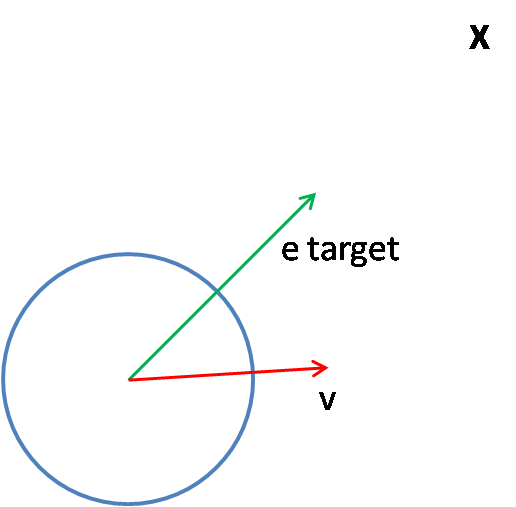
\includegraphics[scale=0.4]{pics/sfm/drivingforce} 
    \par
    \end{centering}
    \caption{\label{fig:driving-force}Driving force}
\end{figure}

The second term is known as the ``Social force''. It's calculated
as follows:

\begin{equation}
    \vec{F}_{S_{i}}=\sum_{j=1,j\ne     i}^{N_{P}}Aexp(-\frac{\epsilon_{ij}}{B})\,\vec{e}_{ij}^{n}\label{eq:social-force}
\end{equation}


$\vec{F}_{S_{i}}$ represents the fact that a pedestrian keeps a certain
distance to other pedestrians and borders.

$N_{p}$ is the number of existing pedestrians.

$A$ and $B$ are constants determined by simulations.

$\epsilon_{ij}$ is the distance from $x_{i}$ towards $x_{j}$.

$\vec{e}_{ij}^{n}$ is the unit vector from $x_{i}$ towards $x_{j}$.\\


Figure \ref{fig:Social-Force} shows \ref{eq:social-force} graphically.

\begin{figure}[h]
    \begin{centering}
    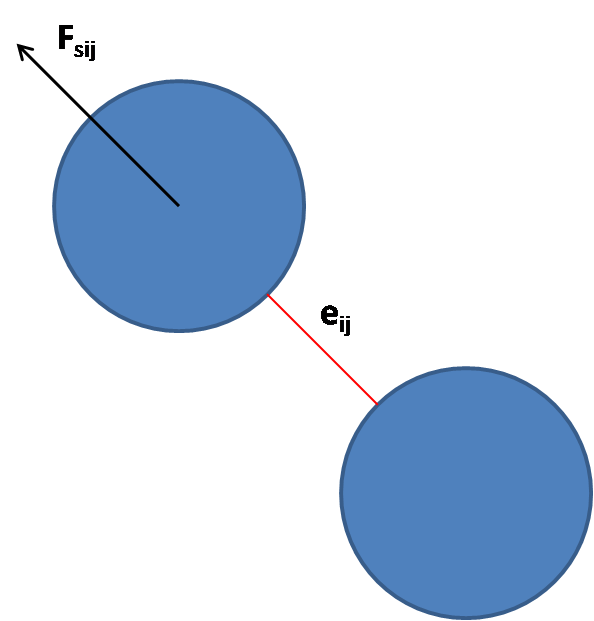
\includegraphics[scale=0.4]{pics/sfm/sf} 
    \par
    \end{centering}
    \caption{Social Force\label{fig:Social-Force}}
\end{figure}

The third term is known as the ``Granular force''. It's calculated
as follows:

\begin{equation}
    \vec{F}_{G_{i}}=\sum_{j=1,j\ne i}^{N_{P}}[-\epsilon_{ij}k_{n}\vec{e}_{ij}^{n}+v_{ij}^{t}\epsilon_{ij}k_{t}\vec{e}_{ij}^{t}]\, g(\epsilon_{ij})\label{eq:granular-force}
\end{equation}


$\vec{F}_{G_{i}}$ represents the physical force that a pedestrian
suffers when colliding with another object (pedestrian or wall).

$k_{n}$ and $k_{t}$ are the normal and tangential friction coeficient
respectively.

$g$ is $0$ if $\epsilon_{ij} \leq 0$  or $\epsilon_{ij}$ otherwise\\

Figure \ref{fig:colliding-pedestrians} shows \ref{eq:granular-force}
graphically.

\begin{figure}[h]
    \begin{centering}
    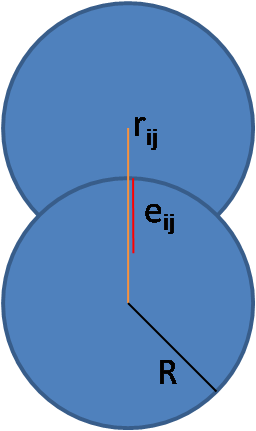
\includegraphics[scale=0.4]{pics/sfm/ganular} 
    \par\end{centering}
    \caption{Colliding pedestrians\label{fig:colliding-pedestrians}}
\end{figure}

Afterwards $\vec{F}_{i}$ is calculated on each simulation step for
each of the pedestrians and applied until all of them had reached
their goal.

Fixed parameter values:

\begin{center}
    \begin{tabular}{|c|c|}
    \hline 
    Name & Value\tabularnewline
    \hline 
    \hline 
    $A$ & $2000\,[N]$\tabularnewline
    \hline 
    $B$ & $0.08\,[m]$\tabularnewline
    \hline 
    $k_{n}$ & $1.2\,10^{5}\,[\frac{N}{m}]$\tabularnewline
    \hline 
    $k_{t}$ & $2.4\,10^{5}\,[\frac{kg}{m/s}]$\tabularnewline
    \hline 
    $\tau$ & $0.5\,[s]$\tabularnewline
    \hline 
    \end{tabular}
    \par
\end{center}


\subsection{Future Virtual Particle Model}

Given that the SFM adds a fictional force on pedestrians, navigation is unnatural and doesn't resemble reality.
SFM isn't validated using well known metrics for real-case scenarios
such as the flow of pedestrians going out a door and the fundamental diagram {Parisi et al. 2009}.

In the FVPM, the social force in equation \ref{eq:driving-force} is eliminated and replaced with a dynamic driving force towards a short term objective, which is equal to \ref{eq:desired-direction} replacing $\vec{x}_{i}^{k}$ with $\vec{x_{i'}}$, where $\vec{x_{i'}}$ is an estimation of the location 
of pedestrian $i$ in the near future. $i'$ will bbe called Future Virtual Particle.

\section{The Model}

\subsection{Hipotesis}

The heuristics that govern the motion of a pedestrian are the same
as Helbin's \cite{key-helb1995,key-helb2000}:

\begin{enumerate}
    \item The pedestrian wants to reach his goal in the shortest possible path. 
    \item The pedestrian's movement is influenced by other pedestrians. Depending
    on the distance between the two of them and the predicted trajectory,
    the pedestrian needs to change his route to be able to avoid
    obstacles.
    \item Movement speed will be influenced by the presence of other pedestrians
and obstacles.
\end{enumerate}

\subsection{Geometrical definition}

A pedestrian is defined as follows: 
\begin{itemize}

    \item Circular shape
    
    Represents the personal space of a pedetrian. The value of the radio
    is generated randomly for each pedestrian. The range of values is
    distributed uniformly in $[0.25,0.29]$ $[cm]$ between pedestrians.
    
    \item Long term target
    
    Represented by a static area. It is considered as accomplished when 
    the pedestrian touches this area. Multiple objectives could be defined
    in a list, in this case, each of them must be reached in order.
    
    \item Short term target
    
    Called future virtual particle (FVP), it represents a point at a relative
    distance from the pedestrian's center. It's a dynamic objective.
    
    
    It is defined as a $1\,[kg]$ mass. Not collisionable.
    
    \item Desired speed
    
    The speed the pedestrian would walk if he/she was alone. This
    represents the constant $v_{di}$ in ecuation \ref{eq:driving-force}.
    It takes a different value for each pedestrian. Varies with a uniform
    distribution between $[1.2,1.4]\,[m/s]$.
    
    \item Reaction distance ($RD$)
    
    Maximum distance between a pedestrian and his FVP, it represents the
    distance at which a real pedestrian would react from an obstacle.

\end{itemize}

\vspace{1cm}

\begin{figure}[!ht]
    \centering{}
    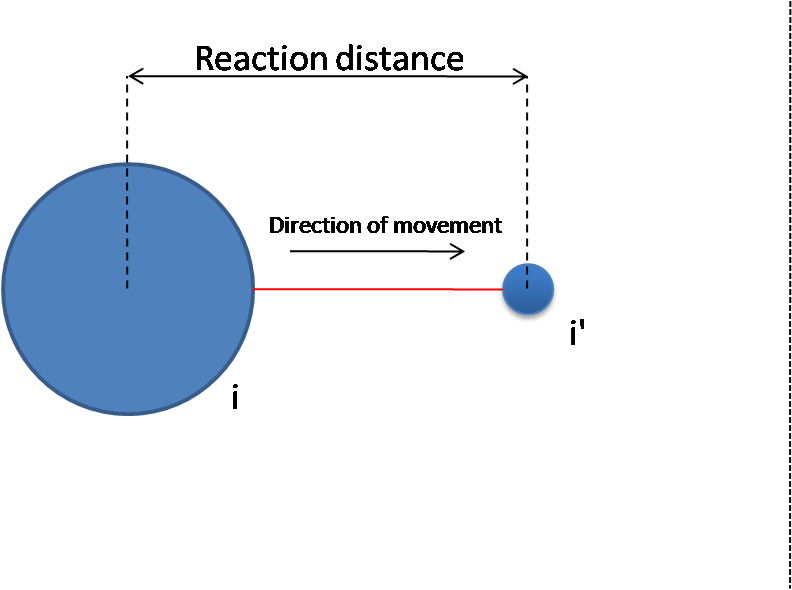
\includegraphics[scale=0.4]{pics/pedestrian-top}
    \caption{\label{fig:pedestrian-geometry}Illustration of pedestrian $i$ and its FVP ($i'$).}
\end{figure}

The naming used is shown in illustration \ref{fig:pedestrian-vectors}.

\begin{figure}[!ht]
    \centering{}
    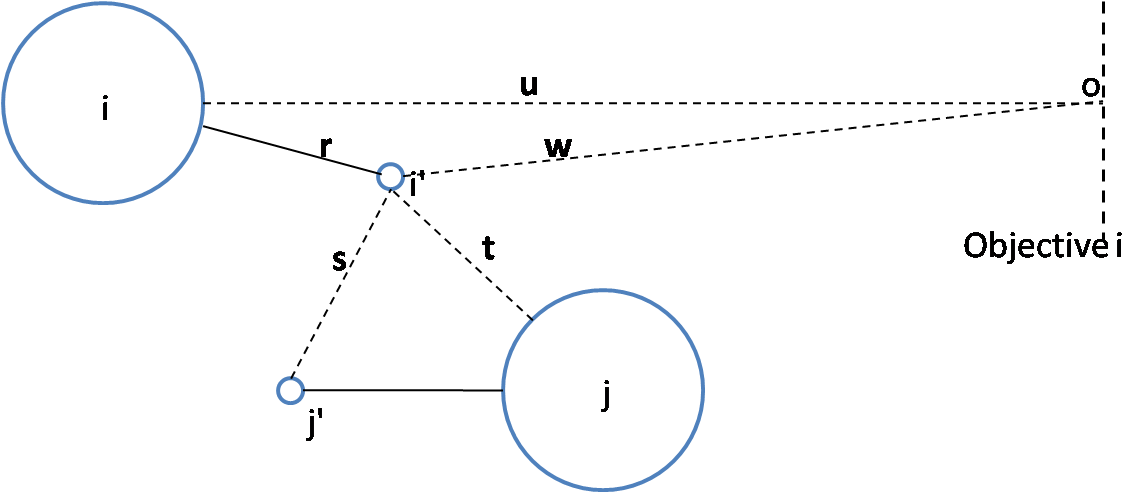
\includegraphics[scale=0.4]{pics/geometry}
    \caption{\label{fig:pedestrian-vectors}Vectorial definitions}
\end{figure}

\subsection{Dynamics}

\subsubsection{Force calculation}
\begin{itemize}
\item Dynamic of the FVP


Each pedestrian has to reach the long term objective at some point,
to ensure this, the FVP needs to be aligned with the shortest path
to the long term objective $\mathbf{x_o}$. On the other hand, there
are sometimes obstacles in the way, which will make this impossible,
in this cases, the route will have to change depending on the situation.


To model this situations, two types of forces act over the FVP:
\begin{itemize}

    \item Internal force \\

     This force will guide the pedestrian on the shortest path $\mathbf{x_{o}x_{i}}$.
    This force is modeled using two springs: 

    The first spring starts on $x_{i}$, ends on $x_{i'}$ and has a stationary
    distance of $RD$ with a spring constant $K_{s}(\theta)$ where $\theta$
    is the angle between $\mathbf{u}$ and $\mathbf{r}$. With this spring
    the FVP will tend to always be at $RD$ distance from the pedestrian.
    Because a pedestrian always tries to reach his goal in the shortest
    possible path (hypothesis 1), if it has to take a big detour of his
    ideal path, it will try to reduce his velocity drastically in order
    to avoid making a long travel. To recreate this, the spring constant
    has to be dependant of the deviation angle. 
    \[
         K_{s}(\theta)=\frac{K_{2}}{\theta}
    \]

    The second spring starts on $x_{i'}$ and ends on 
    $x_i + RD \frac{\vec{x_{i}x_{o}}}{\mid \vec{x_{i}x_{o}} \mid}$
    with a spring constant $K_{1}$.
    This spring represents the pedestrian's desire to reach his
    target. A greater spring constant will force a straighter path.
    In order to avoid an oscillatory movement,
    a damping $\gamma$ was added to the spring.\\

    For any pedestrian $i$, its internal force is

    \begin{equation}
        F_{internal}(i)= F_{S1}(i) + F_{S2}(i)
    \end{equation}
    
    where
    
    \[
        F_{S1}(i) = K_{1} \cdot (|\vec{r}|-RD) \cdot \hat{r}
    \]
    \[
        F_{S2}(i) = \,K_{2}(\theta_{i}) \cdot (\vec{x_{i'}}-(\vec{x_{i}}+\hat{x_{i}o}\cdot RD))
    \]

    \begin{figure}[h]
        \centering{}
        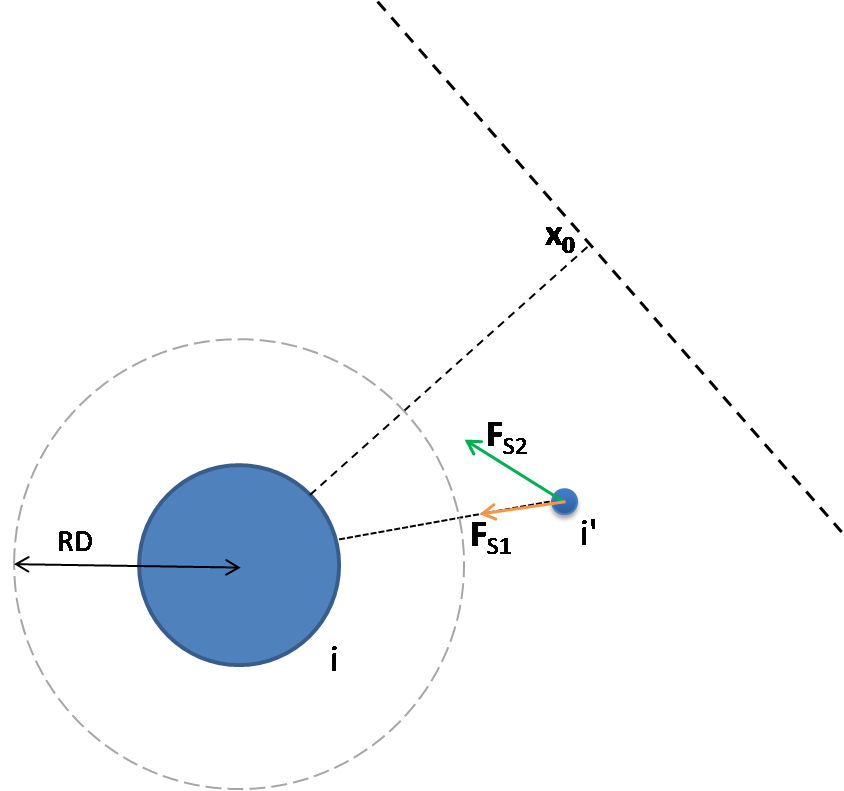
\includegraphics[scale=0.35]{pics/pedestrian-internal-forces}
        \caption{Pedestrian internal forces}
    \end{figure}

    \item Avoidance forces \\
    \\
    This force will produce avoidance movements when obstacles are detected
    on the path. The magnitude of this force is calculated using two factors:
    \\
    The first factor is calculated for each of the pedestrian $j$ ($j\neq i$)
    who is in the range of sight of pedestrian $i$. This restriction
    is verified using the following condition:

    \[
        \mathbf{r_{ii'}}\bullet\mathbf{r_{ij}} < 0
    \]

    This condition represents the fact that pedestrians make decisions 
    based only on obstacles in his range of vision. The formula for the
    external force that affects the FVP $i'$ is
    
    \[
        F_{ext}(i') = FF(i') + FP(i') + FW(i')
    \]
    where
    \[
        FF_(i') = \sum_{j}(\alpha_{ff}e^{-s/\beta_{ff}})
    \]
    \[
        FP_(i') = \sum_{j}(\alpha_{fp}e^{-t/\beta_{fp}})
    \]
    \[
        FW_(i') = \sum_{w}(\alpha_{fw}e^{-dist(w,i')/\beta_{fw}})
    \]

    where $\alpha_{x}$ and $\beta_{x}$ are constants.
    
    The first term of the sum acts as a repulsion force between $i'$ and
    $j'$, resulting in the avoidance of a future collision. The second
    term uses this same principle but calculates the repulsion force between
    $j'$ and $i$. The third term adds the repulsion against walls, using the
    closest point between $i'$ and the wall.
    
    \iffalse The first term of the sum represents the fact that $i$
    does not want to be in the same location as $j$ in the near future.
    Note that $j'$ represents the predicted location of $j$ inferred
    by another pedestrian (in this case, $i$) and because of this, it
    moves it's near future away of that predicted location. The second
    term, represents the same fact but taking in mind the current location
    of the pedestrian $j$. The same law applies to each of the walls
    on the simulation, the difference is that the closest point on the
    wall and and the future has to be calculated before applying the formula.
    Also, the constants $\alpha_{fw}$ and $\beta_{fw}$ have different
    values. \fi

    Figure \ref{fig:External-forces-affecting} shows the external forces
    that a pedestrian $i$ suffers because of another pedestrian ($j$)
    and also the direction in which $i$ desires to move.

    \begin{figure}[!ht]
        \centering{}
        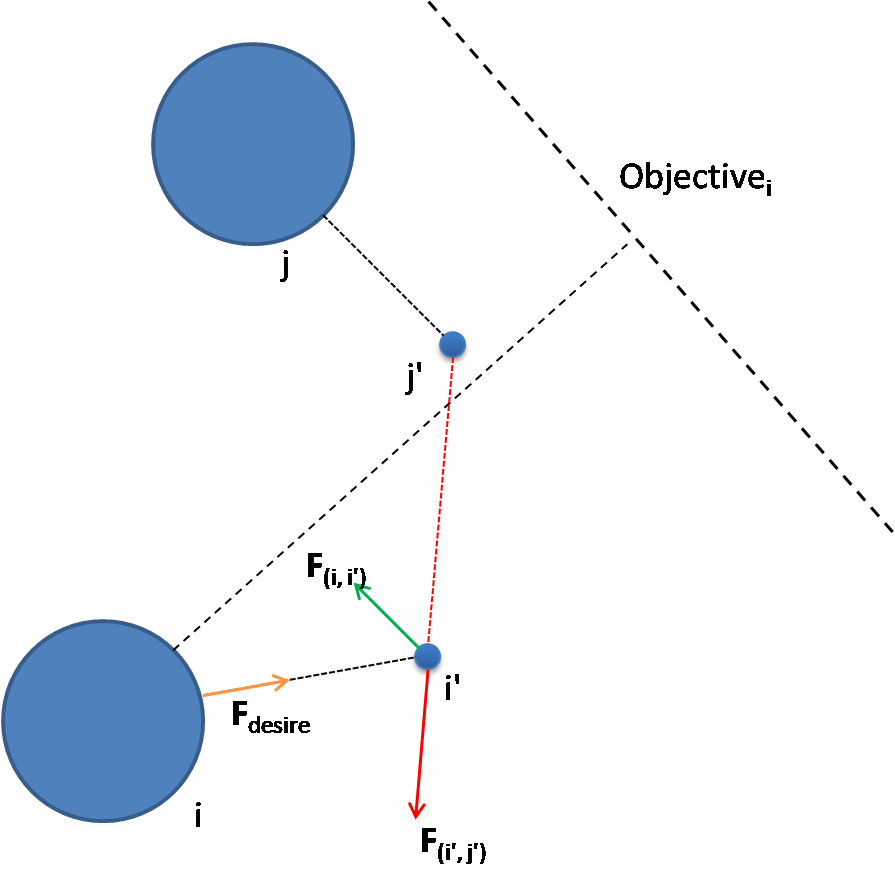
\includegraphics[scale=0.4]{pics/pedestrian-top-forces}
        \caption{\label{fig:External-forces-affecting}External forces affecting future $i'$}
    \end{figure}

\end{itemize}

After this, the final $F_{i'}$ is computed by adding all the terms.
$F_{i'}=F_{ext}(i)+F_{i\, s1}+F_{i\, s2}$.\\



To avoid high symetry situations, a low noise $P=10\%$ is added to
$F$. There are two ways to apply this noise: 
\begin{itemize}
\item Radial noise:

\begin{itemize}
\item A value $p$ is taken randomly from a uniform distribution $[-P,\, P]$
and calculate: $FL_{i'}=F_{i'}*p$ 
\item Angular noise:

\begin{itemize}
\item A value $sgn=\{-1,\,1\}$ is taken randomly from a uniform distribution
and a value $p$ from $[-P,\, P]$. Then $FA_{i'}=rotation(F_{i'},\,\pi*sgn)*p$
is calculated. 
\end{itemize}
\end{itemize}

At last, we find $F'_{i'}=F_{i'}+FL_{i'}+FA_{i'}$ and apply movement
equations.

\end{itemize}
\item Dynamic of the pedestrian


The pedestrian always wants to move in the direction his FVP is pointing
and its magnitude is defined as $F_{d}$ or driving force:


\[
\vec{F}_{desire_{i}}=m_{i}\frac{\frac{|\vec{ii'}|}{|\vec{r}_{max}|}\vec{e_{i}}-\vec{v}_{i}}{\tau}
\]



Where $\tau=0.5$


\textit{{*}It is important to note that the only deviation from the
SFM in this equation is the $k\vec{e}_{i}$ term. As described above,
this model focuses on improving the SFM through dynamically adjusting
the desired velocity.}

\end{itemize}

\subsubsection{Algorithm}

The pedestrian movement is calculated in four steps: 
\begin{enumerate}
    \item Calculate forces for each FVP. 
    \item Update positions for each FVP. 
    \item Calculate forces for each pedestrian. 
    \item Update positions for each pedestrian. 
\end{enumerate}

\section{Calibration}


\subsection{Metrics}

The results where compared to the SFM \cite{key-helb2000}. The test scenarios
where crossing and hallway for they present the main types of symmetry
(90 degrees and 180 degrees respectively).

The metrics used where: 
\begin{enumerate}

    \item Number of collisions
    The total amount of collisions between pedestrians.
    
    \item Total duration of collisions:
    The sum of the duration of each collision.
    
    \item Average walking speed:
    The average of the average speed of each pedestrian.
    
    \item Average travel time:
    The average time that a pedestrian needed unit it reached the goal.
    
    \item Average travel distance:
    The average distance that a pedestrian traveled unit it reached the
    goal.
    
    \item Average turn angle:
    The average angle turned by a pedestrian unit it reached the goal.

\end{enumerate}

\subsection{Values}

To calibrate the model, runs varying parameters were made. A wide
spectrum of values was covered, testing every combination of every
possible one. After seeing clear preferences towards certain values,
the values were refined within that scope. After numerous iterations
of this process, the values that best suit these metrics are:

\begin{itemize}

\item Pedestrian
\begin{itemize}
    \item $K_{1}=100$ {[}N/m{]}, 
    \item $\gamma=10$
    \item $K_{2}=150$ {[}N/m{]}
\end{itemize}

\item FVP-FVP interaction
    \begin{itemize}
        \item $\alpha=1000$
        \item $\beta=[0.4,\,0.5]$ (Uniform distribution)
    \end{itemize}

    \item Pedestrian-FVP interaction
    \begin{itemize}
        \item $\alpha=1000$
        \item $\beta=0.1$
    \end{itemize}
    
    \item FVP-Wall interaction
    \begin{itemize}
        \item $\alpha=10000$
        \item $\beta=0.1$
    \end{itemize}
\end{itemize}

\section{Results}

Metric results for crossing scenario:

\begin{tabular}{|c|c|c|}
    \hline 
    Metric & {\scriptsize{FVPM}} & {\scriptsize{(SFM) $\alpha=2000,\,\beta=0.08$}}\tabularnewline
    \hline 
    \hline 
    $1$ & {\scriptsize{$(1.800,0.748)$}} & {\scriptsize{$(5.333,2.625)$}}\tabularnewline
    \hline 
    $2$ & {\scriptsize{$(34.600,8.333)$}} & {\scriptsize{$(12.333,8.340)$}}\tabularnewline
    \hline 
    $3$ & {\scriptsize{$(1.024,0.016)$}} & {\scriptsize{$(1.052,0.003)$}}\tabularnewline
    \hline 
    $4$ & {\scriptsize{$(1.910,0.022)$}} & {\scriptsize{$(1.876,0.003)$}}\tabularnewline
    \hline 
    $5$ & {\scriptsize{$(2.392,0.005)$}} & {\scriptsize{$(2.391,0.002)$}}\tabularnewline
    \hline 
    $6$ & {\scriptsize{$(91.062,12.122)$}} & {\scriptsize{$(106.185,13.778)$}}\tabularnewline
    \hline 
\end{tabular}

\vspace{1cm}

Metric results for hallway scenario:

\begin{tabular}{|c|c|c|}
    \hline 
    Metric & {\scriptsize{FVPM}} & {\scriptsize{(SFM) $\alpha=2000,\,\beta=0.08$}}\tabularnewline
    \hline 
    \hline 
    $1$ & {\scriptsize{$(24.400, 2.653)$}} & {\scriptsize{$(52.400, 4.543)$}}\tabularnewline
    \hline 
    $2$ & {\scriptsize{$(190.800, 28.701)$}} & {\scriptsize{$(252.800, 28.764)$}}\tabularnewline
    \hline 
    $3$ & {\scriptsize{$(1.237, 0.014)$}} & {\scriptsize{$(1.235, 0.002)$}}\tabularnewline
    \hline 
    $4$ & {\scriptsize{$(0.919, 0.009)$}} & {\scriptsize{$(0.920, 0.003)$}}\tabularnewline
    \hline 
    $5$ & {\scriptsize{$(20.922, 0.132)$}} & {\scriptsize{$(22.823, 0.077)$}}\tabularnewline
    \hline 
    $6$ & {\scriptsize{$(142.495, 11.511)$}} & {\scriptsize{$(160.950, 7.749)$}}\tabularnewline
    \hline 
\end{tabular}

% needed in second column of first page if using \IEEEpubid
%\IEEEpubidadjcol

% An example of a floating figure using the graphicx package.
% Note that \label must occur AFTER (or within) \caption.
% For figures, \caption should occur after the \includegraphics.
% Note that IEEEtran v1.7 and later has special internal code that
% is designed to preserve the operation of \label within \caption
% even when the captionsoff option is in effect. However, because
% of issues like this, it may be the safest practice to put all your
% \label just after \caption rather than within \caption{}.
%
% Reminder: the "draftcls" or "draftclsnofoot", not "draft", class
% option should be used if it is desired that the figures are to be
% displayed while in draft mode.
%
%\begin{figure}[!t]
%\centering
%\includegraphics[width=2.5in]{myfigure}
% where an .eps filename suffix will be assumed under latex, 
% and a .pdf suffix will be assumed for pdflatex; or what has been declared
% via \DeclareGraphicsExtensions.
%\caption{Simulation Results}
%\label{fig_sim}
%\end{figure}

% Note that IEEE typically puts floats only at the top, even when this
% results in a large percentage of a column being occupied by floats.


% An example of a double column floating figure using two subfigures.
% (The subfig.sty package must be loaded for this to work.)
% The subfigure \label commands are set within each subfloat command, the
% \label for the overall figure must come after \caption.
% \hfil must be used as a separator to get equal spacing.
% The subfigure.sty package works much the same way, except \subfigure is
% used instead of \subfloat.
%
%\begin{figure*}[!t]
%\centerline{\subfloat[Case I]\includegraphics[width=2.5in]{subfigcase1}%
%\label{fig_first_case}}
%\hfil
%\subfloat[Case II]{\includegraphics[width=2.5in]{subfigcase2}%
%\label{fig_second_case}}}
%\caption{Simulation results}
%\label{fig_sim}
%\end{figure*}
%
% Note that often IEEE papers with subfigures do not employ subfigure
% captions (using the optional argument to \subfloat), but instead will
% reference/describe all of them (a), (b), etc., within the main caption.


% An example of a floating table. Note that, for IEEE style tables, the 
% \caption command should come BEFORE the table. Table text will default to
% \footnotesize as IEEE normally uses this smaller font for tables.
% The \label must come after \caption as always.
%
%\begin{table}[!t]
%% increase table row spacing, adjust to taste
%\renewcommand{\arraystretch}{1.3}
% if using array.sty, it might be a good idea to tweak the value of
% \extrarowheight as needed to properly center the text within the cells
%\caption{An Example of a Table}
%\label{table_example}
%\centering
%% Some packages, such as MDW tools, offer better commands for making tables
%% than the plain LaTeX2e tabular which is used here.
%\begin{tabular}{|c||c|}
%\hline
%One & Two\\
%\hline
%Three & Four\\
%\hline
%\end{tabular}
%\end{table}




\section{Conclusion}

Pedestrians can adjust their desired velocity at will, based on the data they perceive.
We proposed a model that calculates the desired velocity of the social force model by
conceptually moving the social force into the near future (FVP). The results look
more natural than the original SFM and have been validated with experimental data.
We used real-life metrics to validate our model, the results show that our model
resembles reality with high fidelity.
The proposed model produces a more natural navigation, but, at high densities, this
isn't true, we still need further analysis of this scenario to adjust our model for
both cases. In future work, the paths our virtual pedestrians make need to be compared
and validated with real-life pedestrians paths to complement the use of metrics for the
mean of pedestrians. Parameters should be revalidated with more metrics and analyzed in
more detail.

\newpage

\appendices

\section{Scenarios}

\begin{figure}[!ht]
    \begin{centering}
    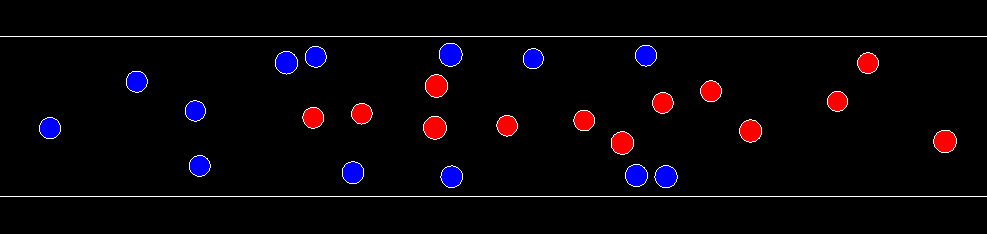
\includegraphics[scale=0.25]{./pics/program/hallway-no-future}
    \par\end{centering}
    \caption{Hallway}
\end{figure}

\begin{figure}[!ht]
    \begin{centering}
    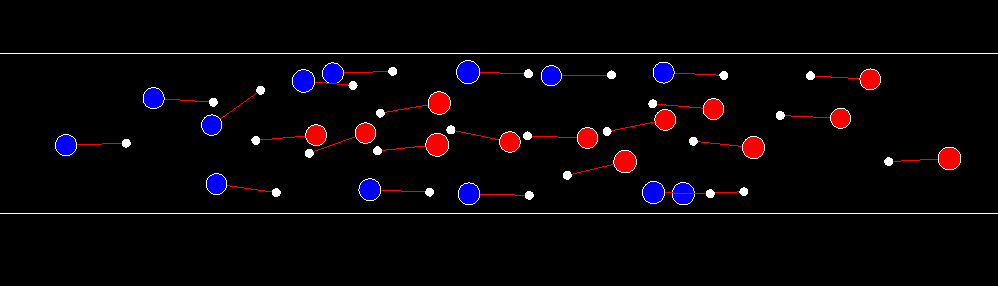
\includegraphics[scale=0.25]{./pics/program/hallway-future}
    \par\end{centering}
    \caption{Hallway with visible future}
\end{figure}


Explain Hallway scenario measures here


\begin{figure}[!ht]
    \begin{centering}
    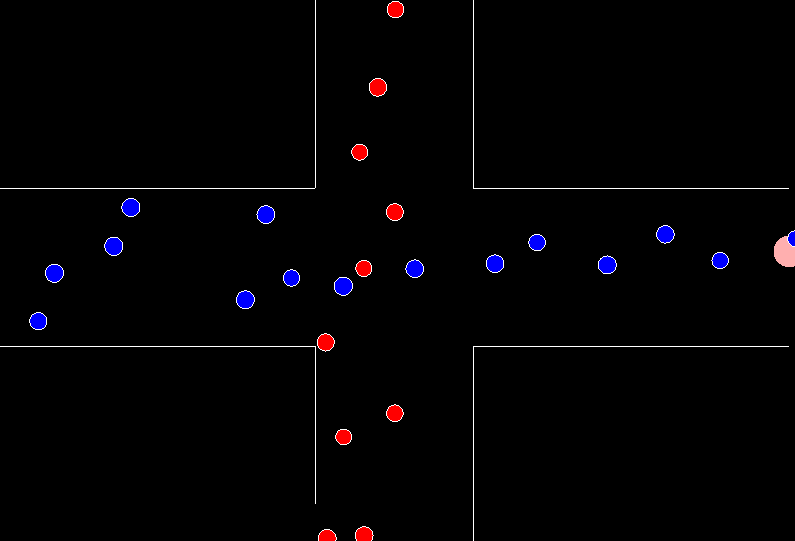
\includegraphics[scale=0.2]{./pics/program/crossing-no-future}
    \par\end{centering}
    \caption{Crossing}
\end{figure}

\begin{figure}[!ht]
    \centering
    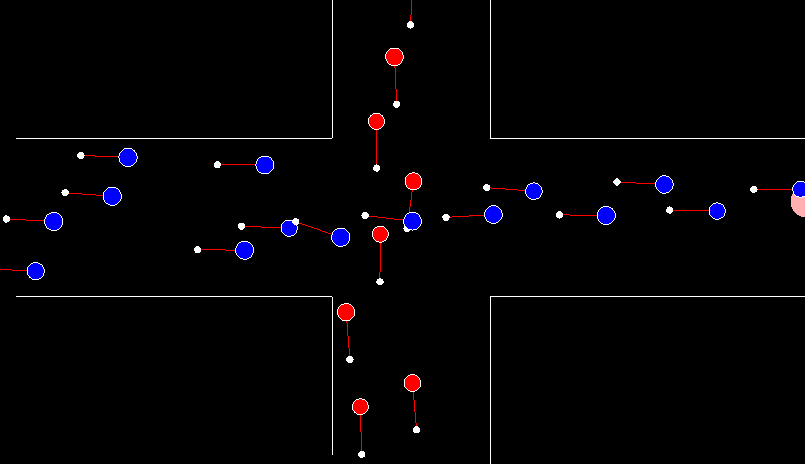
\includegraphics[scale=0.2]{./pics/program/crossing-future}
    \caption{Crossing with visible future}
\end{figure}

Explain Crossing scenario measures here

\begin{figure}[!ht]
    \begin{centering}
    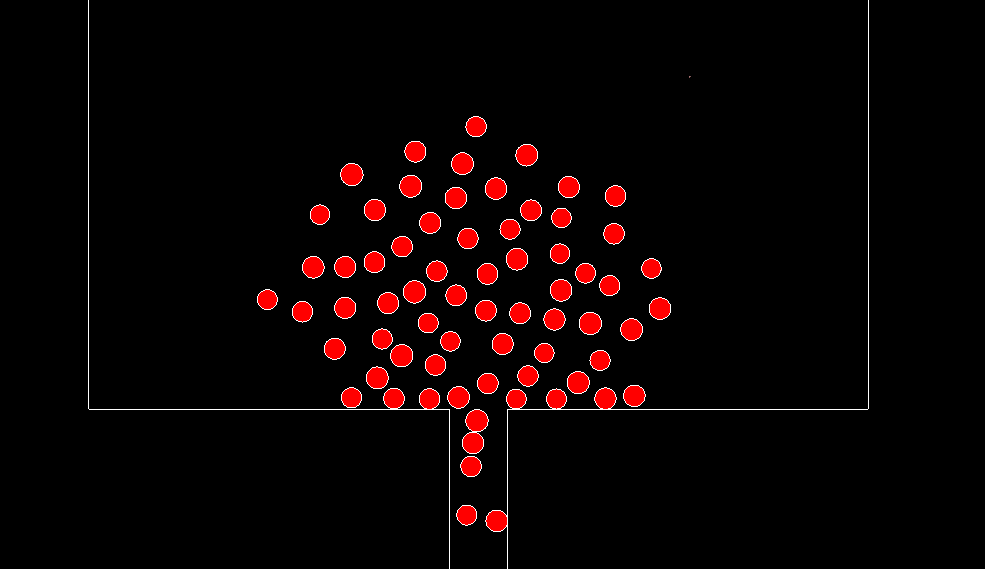
\includegraphics[scale=0.25]{./pics/program/room-no-future}
    \par\end{centering}
    \caption{Room}
\end{figure}

\begin{figure}[!ht]
    \centering
    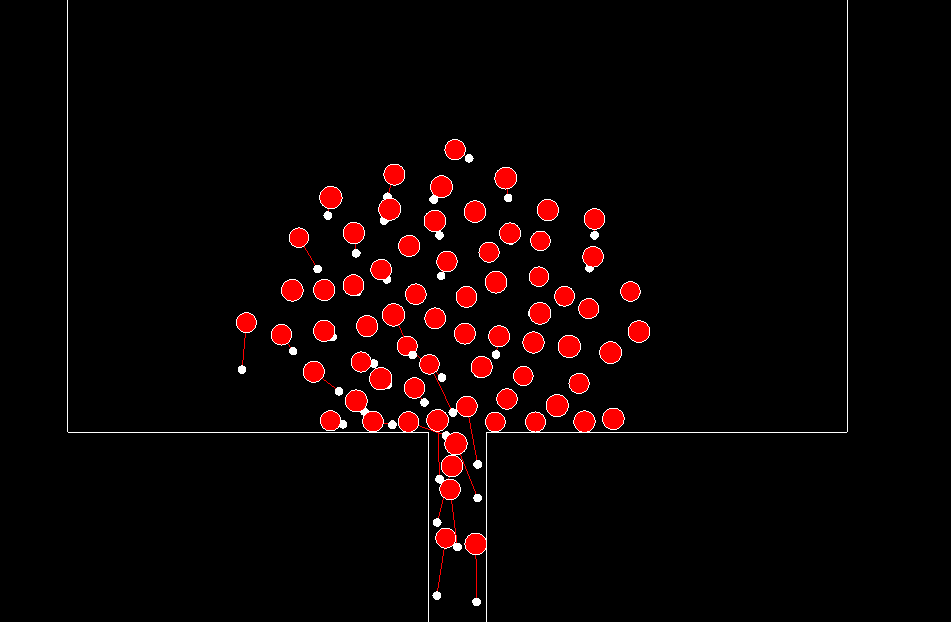
\includegraphics[scale=0.25]{./pics/program/room-future}
    \caption{Room with visible future}
\end{figure}

Explain Room scenario measures here

\section*{Acknowledgment}
The authors would like to thank Daniel Parisi, ITBA, .... for ....

\vfill

\begin{thebibliography}{1}

\bibitem{key-hoog2004} Hoogonen and Bovy (2004).
\bibitem{key-scha2009} A. Schadschneider (2009). "Evacuation Dynamics: Empirical Results, Modeling and Applications".
\bibitem{key-scha2002} A. Schadschneider (2009). "Traffic flow: A statistical physics point of view".
\bibitem{key-helb1995} Helbing, Dirk; Molnr, Pter (1995). “Social force model for pedestrian dynamics”.
\bibitem{key-helb2000} Helbing, Dirk; Farkas, Ills; Vicsek, Tams (2000). “Simulating dynamical features of escape panic”.
\bibitem{key-tara2005} Taras I. Lakoba (2005). "Modifications of the Helbing-Molnár-Farkas-Vicsek Social Force Model for Pedestrian Evolution".
\bibitem{key-pari2009} Parisi (2009). "A modification of the Social Force Model can reproduce experimental data of pedestrian flows in normal conditions".
\bibitem{key-kirc2002} Kirchner and Schadschneider (2002). "Simulation ofevacuation processes using a bionics-inspired cellular automaton model for pedestrian dynamics".
\bibitem{key-pari2011} Baglietto and Parisi, (2011). "Continuous-space automaton model for pedestrian dynamics".
\bibitem{key-kara2009} I. Karamouzas (2009). "A Predictive Collision Avoidance Model for Pedestrian Simulation".
\bibitem{key-kret2001} Kretz (2011). "Quickest Paths in Simulations of Pedestrians".
\bibitem{key-mous2009} Moussad M, Helbing D, Garnier S, Johansson A, Combe M and aulaz G (2009).


\end{thebibliography}



\end{document}


